%% Based on a TeXnicCenter-Template by Gyorgy SZEIDL.
%%%%%%%%%%%%%%%%%%%%%%%%%%%%%%%%%%%%%%%%%%%%%%%%%%%%%%%%%%%%%

%----------------------------------------------------------
%
\documentclass{report}%
%
%----------------------------------------------------------
% This is a sample document for the standard LaTeX Report Class
% Class options
%       --  Body text point size:
%                        10pt (default), 11pt, 12pt
%       --  Paper size:  letterpaper (8.5x11 inch, default)
%                        a4paper, a5paper, b5paper,
%                       legalpaper, executivepaper
%       --  Orientation (portrait is the default):
%                       landscape
%       --  Printside:  oneside (default), twoside
%       --  Quality:    final (default), draft
%       --  Title page: titlepage, notitlepage
%       --  Columns:    onecolumn (default), twocolumn
%       --  Start chapter on left:
%                       openright(no), openany (default)
%       --  Equation numbering (equation numbers on right is the default)
%                       leqno
%       --  Displayed equations (centered is the default)
%                       fleqn (flush left)
%       --  Open bibliography style (closed bibliography is the default)
%                       openbib
% For instance the command
%          \documentclass[a4paper,12p,leqno]{report}
% ensures that the paper size is a4, fonts are typeset at the size 12p
% and the equation numbers are on the left side.
%
\usepackage{amsmath}%
\usepackage{amsfonts}%
\usepackage{amssymb}%
\usepackage{graphicx}
%----------------------------------------------------------
\usepackage{url}
\usepackage[square,sort,comma,numbers]{natbib}
\usepackage{chapterbib}
\usepackage{hyperref}
\usepackage{url}
\usepackage{doi}
\usepackage{listings}
\usepackage{color}
%----------------------------------------------------------
% Define colors:
\definecolor{dkgreen}{rgb}{0,0.6,0}
\definecolor{gray}{rgb}{0.5,0.5,0.5}
\definecolor{mauve}{rgb}{0.58,0,0.82}
% Define language
\lstdefinelanguage{torxakis}
{
  % list of keywords
  morekeywords={
    PROCDEF,
    FUNCDEF
  },
  sensitive=false, % keywords are not case-sensitive
  morecomment=[l]{//}, % l is for line comment
  morecomment=[s]{/*}{*/}, % s is for start and end delimiter
  morestring=[b]" % defines that strings are enclosed in double quotes
}
% Define environment:
\lstset{frame=tb,
  language=torxakis,
  aboveskip=3mm,
  belowskip=3mm,
  showstringspaces=false,
  columns=flexible,
  basicstyle={\small\ttfamily},
  numbers=none,
  numberstyle=\tiny\color{gray},
  keywordstyle=\color{blue},
  commentstyle=\color{dkgreen},
  stringstyle=\color{mauve},
  breaklines=true,
  breakatwhitespace=true,
  tabsize=3
}
%----------------------------------------------------------
\newcommand{\txs}{TorXakis}
\newcommand{\inlinecode}[1]{{\lstinline[language=torxakis]{#1}}}
%----------------------------------------------------------
\newtheorem{theorem}{Theorem}
\newtheorem{acknowledgement}[theorem]{Acknowledgement}
\newtheorem{algorithm}[theorem]{Algorithm}
\newtheorem{axiom}[theorem]{Axiom}
\newtheorem{case}[theorem]{Case}
\newtheorem{claim}[theorem]{Claim}
\newtheorem{conclusion}[theorem]{Conclusion}
\newtheorem{condition}[theorem]{Condition}
\newtheorem{conjecture}[theorem]{Conjecture}
\newtheorem{corollary}[theorem]{Corollary}
\newtheorem{criterion}[theorem]{Criterion}
\newtheorem{definition}[theorem]{Definition}
\newtheorem{example}[theorem]{Example}
\newtheorem{exercise}[theorem]{Exercise}
\newtheorem{lemma}[theorem]{Lemma}
\newtheorem{notation}[theorem]{Notation}
\newtheorem{problem}[theorem]{Problem}
\newtheorem{proposition}[theorem]{Proposition}
\newtheorem{remark}[theorem]{Remark}
\newtheorem{solution}[theorem]{Solution}
\newtheorem{summary}[theorem]{Summary}
\newenvironment{proof}[1][Proof]{\textbf{#1.} }{\ \rule{0.5em}{0.5em}}
%----------------------------------------------------------
\begin{document}

\title{LPE operations}
\author{Djurre van der Wal}
\date{\today}
\maketitle
\tableofcontents

\chapter{LPE structure}

\section{Introduction}
The LPE operations that are described in this document (see \ref{lpeoperations}) require a \txs{} model as input of which the process is in \emph{linear process equation} (LPE) \emph{form}.
Many, but not all \txs{} processes can be transformed to LPE form using the \texttt{lpe} command of \txs{}.

\section{LPE form} \label{lpeform}

A \txs{} process
\begin{align*}
\texttt{ProcDef} \; [C_1 :: K_1, \cdots{}, C_n :: K_n] \; [p_1 :: T_1, \cdots{}, p_k :: T_k] \; b_\textit{LPE}
\end{align*}

that is identified by $P$ is said to be a in \emph{LPE form} if $b_\textit{LPE}$ follows the grammar of $\textit{LPEBody}$ below:
\begin{align*}
\textit{LPEBody} &::= \textit{ChoiceSmd} \\
\textit{ChoiceSmd} &::= \texttt{Choice} \; [ \;\! \textit{ActionSmd}, \cdots{}, \textit{ActionSmd} \; ] \\
\textit{ActionSmd} &::= \texttt{ActionPref} \; \textit{ActOffer} \; \textit{ProcInst} \\
\textit{ActOffer} &::= \texttt{ActOffer} \; \textit{ChanOffers} \;\; [ \; h_1, \cdots{}, h_z \; ] \; \textit{VExpr} \\
\textit{ChanOffers} &::= [ \;\! \textit{ChanOffer}, \cdots{}, \textit{ChanOffer} \; ] \\
\textit{ChanOffer} &::= \textit{ChanId} \;\; [\texttt{Quest} \; x_1, \cdots{}, \texttt{Quest} \; x_m] \\
\textit{ChanId} &::= C_1 \;| \cdots{} |\; C_n \;|\; \texttt{ISTEP} \;|\; \texttt{CISTEP} \\
\textit{ProcInst} &::= \texttt{ProcInst} \; P \; \; [ \; C_1, \cdots{}, C_n \; ] \; [\;\!\textit{VExpr}, \cdots{}, \textit{VExpr} \; ]
\end{align*}

Note that
\begin{itemize}
\item $b_\textit{LPE}$ should comply with traditional \txs{} requirements.
More precisely, the communication variables $\{ x_1, \cdots{}, x_m \}$ must match the signature of the \textit{ChanId} channel that occurs in the same rule; and the number of \textit{VExpr}s in the \textit{ProcInst} rule must be equal to $k$ and their sorts must match $[T_1, \cdots{}, T_k]$.
\item it must be the case that the channels that are used in a summand are either all input channels or all output channels.
\item per summand, it must be the case that
\begin{align*}
|\; \{ h_1, \cdots{}, h_z \} \cup \{ x_1, \cdots{}, x_m \} \; | &= z + m \\
(\{ h_1, \cdots{}, h_z \} \cup \{ x_1, \cdots{}, x_m \}) \cap \{ p_1, \cdots{}, p_k \} &= \emptyset{}
\end{align*}
\end{itemize}

\section{Restricted LPE form} \label{restrictedlpeform}

In actuality, it is convenient that processes have a form that is even more restrictive than the LPE form discussed in \ref{lpeform}.
The form is the same as before, except for the \textit{ActOffer} and \textit{ChanOffers} rules, which change to
\begin{align*}
\textit{ActOffer} &::= \texttt{ActOffer} \; \textit{ChanOffers} \;\; [\;] \; \textit{VExpr} \\
\textit{ChanOffers} &::= [ \;\! \textit{ChanOffer} \; ]
\end{align*}

In short, hidden variables are no longer permitted, and there must be exactly one \textit{ChanOffer} per summand.

A process that is in LPE form can be converted to restricted LPE form in a way that is reversible.
First, a more precise definition of the format of \txs{} models is required.

Let the form of a \txs{} model $M$ be
\begin{align*}
\texttt{ModelDef} \; [I_1, \cdots{}, I_m] \; [O_1, \cdots{}, O_n] \; b_\textit{inst}
\end{align*}

where

\begin{itemize}
\item $I_1, \cdots{}, I_m$ are all single input channels;
\item $O_1, \cdots{}, O_n$ are all single output channels;
\item $b_\text{\textit{inst}}$ has the form
\begin{align*}
\texttt{ProcInst} \; P \; [D_1, \cdots{}, D_{m+n}] \; [v_I(p_1), \cdots{}, v_I(p_k)]
\end{align*}

such that
\begin{align*}
\{ I_1, \cdots{}, I_m \}, \{ O_1, \cdots{}, O_n \} \subseteq \{ D_1, \cdots{}, D_{m+n} \}
\end{align*}

and
\begin{align*}
\{ I_1, \cdots{}, I_m \} \cap \{ O_1, \cdots{}, O_n \} = \emptyset{}
\end{align*}

\item the \txs{} process that is identified by $P$ is
\begin{align*}
\texttt{ProcDef} \; [C_1 :: K_1, \cdots{}, C_{m+n} :: K_{m+n}] \; [p_1 :: T_1, \cdots{}, p_k :: T_k] \; b_\textit{LPE}
\end{align*}
such that
\begin{align*}
\sortof{C_i} = \sortof{D_i} = K_i &\text{ for all } i \in [1, \cdots{}, m+n] \\
\sortof{v_I(p_i)} = T_i &\text{ for all } i \in [1, \cdots{}, k]
\end{align*}

and such that $b_\textit{LPE}$ follows the parametrized grammar of $\textit{LPEBody}$ below:
\begin{align*}
\textit{LPEBody} &::= \textit{ChoiceSmd} \\
\textit{ChoiceSmd} &::= \texttt{Choice} \; [ \;\! \textit{ActionSmd}(1), \cdots{}, \textit{ActionSmd}(s) \; ] \\
\textit{ActionSmd}(i) &::= \texttt{ActionPref} \; \textit{ActOffer}(i) \; \textit{ProcInst}(i) \\
\textit{ActOffer}(i) &::= \texttt{ActOffer} \; \textit{ChanOffers}(i) \; [ \; h_i(1), \cdots{}, h_i(z_i) \; ] \; g_i \\
\textit{ChanOffers}(i) &::= [ \;\! \textit{ChanOffer}_i(1), \cdots{}, \textit{ChanOffer}_i(m_i) \; ] \\
\textit{ChanOffer}_i(j) &::= c_i(j) \;\; [\texttt{Quest} \; x_{i,j}(1), \cdots{}, \texttt{Quest} \; x_{i,j}(|\flsortof{c_i(j)}|)] \\
\textit{ProcInst}_i(j) &::= \texttt{ProcInst} \; P \; \; [ \; C_1, \cdots{}, C_{m+n} \; ] \; [\;\!v_i(p_1), \cdots{}, v_i(p_k) \; ]
\end{align*}

where

\begin{itemize}
\item $s$ is the number of summands of $P$;
\item $h_i(j)$ is the $j$th hidden variable of the $i$th summand of $P$;
\item $z_i \geq 0$ is the number of hidden variables of the $i$th summand of $P$;
\item $g_i$ is the guard of the $i$th summand of $P$;
\item $m_i \geq 0$ is the number of channels over which the $i$th summand of $P$ communicates;
\item $c_i(j)$ is the $j$th channel over which the $i$th summand of $P$ communicates;
\item $\text{fl}(S_1 \; \texttt{\#\#} \cdots{} \texttt{\#\#} \; S_q) = [S_1, \cdots{}, S_q]$ for some $q > 0$;
\item $x_{i,j}(e)$ is the $e$th parameter that the $i$th summand of $P$ uses to communicate over channel $c_i(j)$;
\item $v_i(p)$ is an expression that defines the new value of parameter $p$ of $P$ after the application of summand $s_i$.
\end{itemize}
\end{itemize}

Define a \emph{channel signature} as a pair $(C, S)$ where $C$ is an ordered list of channels and $S$ is an ordered list of sorts, and define a function $\tau$ that yields the channel signature of the $i$th summand of $P$, namely $s_i$:
\begin{align*}
\tau(s_i) = (&[ c_i(1), \cdots{}, c_i(m_i)], \\
&[\flsortof{c_i(1)}, \cdots{}, \flsortof{c_i(m_i)}, \sortof{h_i(1)}, \cdots{}, \sortof{h_i(z_i)}])
\end{align*}

Also define an injective function $\theta(T)$ that maps channel signatures of the form
\begin{align*}
T = (C, [S_1, \cdots{}, S_{m_i+z_i}])
\end{align*}

to a fresh, uniquely named channel with sort $S_1 \; \texttt{\#\#} \cdots{} \texttt{\#\#} \; S_{m_i+z_i}$.

Given these definitions, do the following:

\begin{enumerate}
\item For each summand $s_i$, compute $\tau(s_i)$.
Add the result to a set $\Sigma_I$ if summand $s_i$ contains input actions, or add the result to a set $\Sigma_O$ if summand $s_i$ contains output actions (only one of these can be true).

\item Compute $\Omega_I = \{ \; (\sigma, \theta(\sigma)) \;|\; \sigma \in \Sigma_I \; \}$ and $\Omega_O = \{ \; (\sigma, \theta(\sigma)) \;|\; \sigma \in \Sigma_O \; \}$.

\item Compute $\Theta = [ \; \Theta_1, \cdots{}, \Theta_t \; ] = [ \; b \;|\; (a, b) \in \Omega_I \cup \Omega_O \; ]$.

\item For each summand $s_i$, look up a pair $(a, b) \in \Omega_I \cup \Omega_O$ so that $a = \tau(s_i)$.
There is exactly one such pair.
Change the form of $s_i$ to
\begin{align*}
\textit{ActionSmd}(i) &::= \texttt{ActionPref} \; \textit{ActOffer}(i) \; \textit{ProcInst}(i) \\
\textit{ActOffer}(i) &::= \texttt{ActOffer} \; \textit{ChanOffers}(i) \;\; [ \; ] \;\; g_i \\
\textit{ChanOffers}_i &::= [ \; b \;\; [ \;\! \textit{ChanOffer}_i(1), \cdots{}, \textit{ChanOffer}_i(m_i), \\
&\qquad \qquad \qquad \texttt{Quest} \; h_i(1), \cdots{}, \texttt{Quest} \; h_i(z_i) \; ] \; ] \\
\textit{ChanOffer}_i(j) &::= \texttt{Quest} \; x_{i,j}(1), \cdots{}, \texttt{Quest} \; x_{i,j}(|\flsortof{c_i(j)}|) \\
\textit{ProcInst}_i(j) &::= \texttt{ProcInst} \; P \; \; [ \; \Theta_1, \cdots{}, \Theta_t \; ] \; [\;\!v_i(p_1), \cdots{}, v_i(p_k) \; ]
\end{align*}

\item Change the definition of $P$ to
\begin{align*}
\texttt{ProcDef} \; [\Theta_1 :: \sortof{\Theta_1}, \cdots{}, \Theta_t :: \sortof{\Theta_t}] \; [p_1 :: T_1, \cdots{}, p_k :: T_k] \; b_\textit{LPE}
\end{align*}

\item Change the definition of $M$ to
\begin{align*}
\texttt{ModelDef} \; [ \; b \;|\; (a, b) \in \Omega_I \; ] \; [ \; b \;|\; (a, b) \in \Omega_O \; ] \; b_\textit{inst}
\end{align*}

where
\begin{align*}
b_\textit{inst} = \texttt{ProcInst} \; P \; [\Theta_1, \cdots{}, \Theta_t] \; [v_I(p_1), \cdots{}, v_I(p_k)]
\end{align*}
\end{enumerate}

Given $\Omega_I$ and $\Omega_O$, how to reverse the conversion above should be obvious.

\section{Data structure}

The implementation stores a \txs{} model that is in LPE form in a dedicated data structure before any of the techniques that are described in this document are applied.
A visual representation of this data structure can be found in Figure~\ref{lpedatastructure:fig}.

\begin{figure}[!ht]
\begin{center}
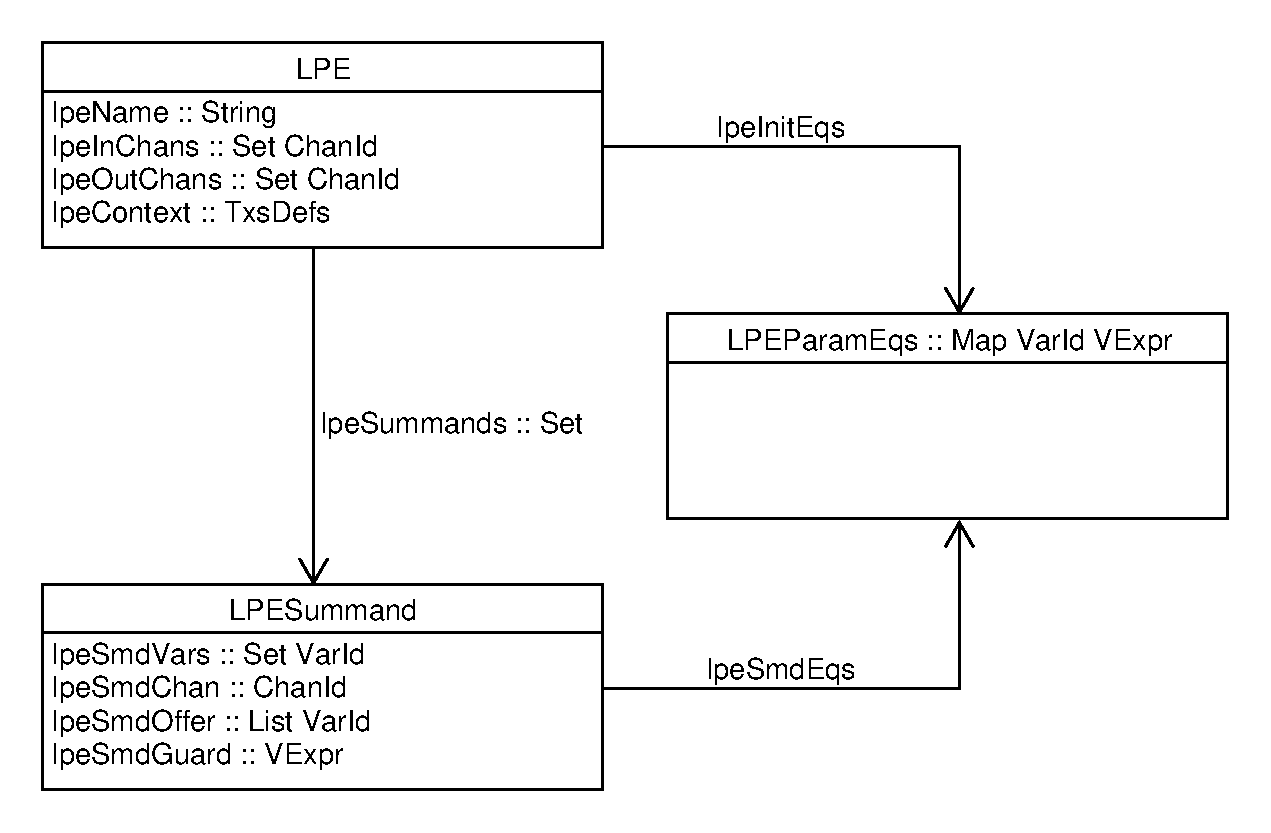
\includegraphics[width=0.7\linewidth]{images/lpe-types}
\caption{LPE data structure.}
\label{lpedatastructure:fig}
\end{center}
\end{figure}

The main data type is \texttt{LPE}.
This type primarily contains information about the \txs{} process in restricted LPE form (see \ref{restrictedlpeform}):
\begin{itemize}
\item The name of the LPE process is \texttt{lpeName};
\item The summands that form the body of the LPE process; and
\item The sorts of the data parameters of the LPE process are contained in \texttt{lpeInitEqs} as well as how each data parameter is initialized.
\end{itemize}

Because the LPE process is always instantiated with the same channels in the same order, the \texttt{LPE} type only has to track which channels are input channels (\texttt{lpeInChans}) and which channels are output channels (\texttt{lpeOutChans}).
Note that these are single channel identifiers that may have been freshly generated from multi-channel summands or from summands with hidden variables in order to obtain restricted LPE form (see \ref{restrictedlpeform}).
The \texttt{lpeChanMap} defines how channels in the LPE data structure are converted back to the original channels; it is therefore the implementation of $\Omega_I$ and $\Omega_O$.

The \texttt{LPE} type also stores some circumstantial information in \texttt{lpeContext}.
This is a library of \txs{} type and function definitions that has been copied directly from the original \txs{} model specification.
It is used to validate instances of the \texttt{LPE} type, to generate default values of a specific sort, and more.

Finally, the \texttt{LPESummand} type only contains information about a specific summand: \texttt{lpeSmdChan} is the channel over which it communicates; \texttt{lpeSmdOffers} are the communication variables (including variables that originally were hidden variables); and the \texttt{lpeSmdEqs} map defines which expressions are used to assign new values to the parameters of the LPE after the application of the summand.

\section{Summand elements} \label{summandelements}

To formally reference the elements of $s_i$ -- the $i$th summand of restricted LPE $P$ -- the following definition is used:
\begin{align*}
s_i = C_i \; \texttt{?} \; x_i(1) \; \cdots{} \; \texttt{?} \; x_i(m_i) \; [[g_i]] \text{ \texttt{>->} } P(v_i(p_1), \cdots{}, v_i(p_k))
\end{align*}

where

\begin{itemize}
\item $C_i$ is the name of the channel over which summand $s_i$ communicates;
\item $m_i \geq 0$ is the number of variables that summand $s_i$ uses to communicate over channel $C_i$;
\item $x_i(j)$ is the $j$th variable that summand $s_i$ uses locally (communication variables first, followed by hidden variables);
\item $g_i$ is the guard of summand $s_i$ (the only free variables in this expression must be parameters of $P$, communication variables of summand $s_i$, or hidden variables of summand $s_i$);
\item $p_1, \cdots{}, p_k$ are the parameters of $P$, of which there are $k \geq 0$;
\item $v_i(p)$ is an expression that defines the new value of parameter $p$ of $P$ after the application of summand $s_i$ (the only free variables in this expression must be LPE parameters, communication variables of summand $s_i$, or hidden variables of summand $s_i$).
\end{itemize}


\chapter{constElm}

\section{Introduction}

A linearized process may have parameters that do not change value throughout the state space of that process.
These parameters are essentially \emph{constants}.

Constants can be removed from a process as follows:
\begin{itemize}
\item Substitute references to a constant by the explicit value of that constant;
\item Remove the constant from the process parameter list.
\end{itemize}

The advantages of removing constants from a process are smaller state vectors (and therefore reduced memory usage) and faster performance in general.
These advantages may be small; however, the detection and removal of constants can be done fairly cheaply.

\section{Algorithm}

The algorithm consists of the following steps \cite{groote2001computer}:

\begin{enumerate}

\item Mark all process parameters.
(This means that, initially, we assume that all process parameters are constants.)

\item Let $P$ be the set of all marked process parameters.
Define a substitution $\rho = [p \rightarrow v_0(p) \;|\; p \in P]$, where $v_0$ is a function that gives the initial value of a given process parameter.

\item Consider each summand $s$ of the LPE.
Construct an equation $c_s \rightarrow p = v_s(p)$ for all $p \in P$, where $c_s$ is the guard of $s$ and where $v_s$ is a function that gives the expression of which the value is assigned to the process parameter $p$ in the instantiation, and apply the substitution $\rho$ to it.
(This gives $(c_s \rightarrow p = v_s(p))[\rho] \Leftrightarrow {c_s}[\rho] \rightarrow v_0(p) = v_s(p)[\rho]$.)

If the obtained equation is a tautology (that is, if its negation is unsatisfiable) for all $s$, $p$ remains marked; otherwise, unmark $p$.

\item Repeat the previous two steps until $P$ remains constant.
All remaining marked process parameters can be safely removed the process.

\end{enumerate}

\section{Example}

Consider the following LPE:

\begin{lstlisting}
//Process definition:
PROCDEF example[A](x, y, z :: Int)
  = A [[z = 2]] >-> example[A](z-1, 1, 2)
  + A >-> example[A](y, x, x+y)
  + A >-> example[A](1, x, z+1)
  ;

//Initialization:
example[A](1, 1, 2);
\end{lstlisting}

First, $\rho = [ x \rightarrow 1, y \rightarrow 1, z \rightarrow 2 ]$.

We must check the following equations:

\begin{align*}
(z = 2 \rightarrow x = z-1)[\rho] &\Leftrightarrow (2 = 2 \rightarrow 1 = 2-1) \Leftrightarrow \textit{true} \\
(z = 2 \rightarrow y = 1)[\rho] &\Leftrightarrow (2 = 2 \rightarrow 1 = 1) \Leftrightarrow \textit{true} \\
(z = 2 \rightarrow z = 2)[\rho] &\Leftrightarrow (2 = 2 \rightarrow 2 = 2) \Leftrightarrow \textit{true} \\
(x = y)[\rho] &\Leftrightarrow (1 = 1) \Leftrightarrow \textit{true} \\
(y = x)[\rho] &\Leftrightarrow (1 = 1) \Leftrightarrow \textit{true} \\
(z = x+y)[\rho] &\Leftrightarrow (2 = 1+1) \Leftrightarrow \textit{true} \\
(x = 1)[\rho] &\Leftrightarrow (1 = 1) \Leftrightarrow \textit{true} \\
(y = x)[\rho] &\Leftrightarrow (1 = 1) \Leftrightarrow \textit{true} \\
(z = z+1)[\rho] &\Leftrightarrow (2 = 2+1) \Leftrightarrow \textit{false} \\
\end{align*}

The last equation is not a tautology, and so $z$ is unmarked.

The new value of $\rho$ is $[ x \rightarrow 1, y \rightarrow 1 ]$.

\clearpage
The equations are now the following:

\begin{align*}
(z = 2 \rightarrow x = z-1)[\rho] &\Leftrightarrow (z = 2 \rightarrow 1 = z-1) \Leftrightarrow \textit{true} \\
(z = 2 \rightarrow y = 1)[\rho] &\Leftrightarrow (z = 2 \rightarrow 1 = 1) \Leftrightarrow \textit{true} \\
(x = y)[\rho] &\Leftrightarrow (1 = 1) \Leftrightarrow \textit{true} \\
(y = x)[\rho] &\Leftrightarrow (1 = 1) \Leftrightarrow \textit{true} \\
(x = 1)[\rho] &\Leftrightarrow (1 = 1) \Leftrightarrow \textit{true} \\
(y = x)[\rho] &\Leftrightarrow (1 = 1) \Leftrightarrow \textit{true} \\
\end{align*}

All of the equations above are tautologies, and so $x$ and $y$ remain marked.
Removing the marked parameters from the LPE gives

\begin{lstlisting}
//Process definition:
PROCDEF example[A](z :: Int)
  = A [[z==2]] >-> example[A](2)
  + A >-> example[A](2)
  + A >-> example[A](z+1)
  ;

//Initialization:
example[A](2);
\end{lstlisting}

Obviously, more simplification is possible.


\chapter{parelm}

\section{Introduction}

An LPE may have parameters that do not affect the behavior of that process in any way.
These parameters are said to be \emph{inert}.
Removing inert parameters from an LPE reduces the size of state vectors and the state space of that LPE, which both benefits performance.

\section{Implementation}

The algorithm consists of the following steps \cite{groote2001computer}:

\begin{enumerate}

\item Make it so that all parameters of the LPE are \labeledas{inert}.

\item Consider the guards of all summands of the LPE, and \removelabelfrom{inert} from all LPE parameters that occur in the guard of a summand.

\item Let $X$ be the set of all LPE parameters that are \labeledas{inert}, and consider all expressions $v_s(p)$ that define the value of an LPE parameter $p$ after application of a summand $s$.
For each such expression, if $p$ is \emph{not} \labeledas{inert}, \removelabelfrom{inert} all LPE parameters that occur in $v_s(p)$.

\item Repeat the previous step until the fixpoint of $X$ is reached.
Then remove all LPE parameters that are still \labeledas{inert} from the LPE, substituting references to those parameters by their initial values.

\end{enumerate}

\clearpage
\section{Example}

Consider the following LPE:

\begin{lstlisting}
//Process definition:
PROCDEF example[A :: Int, B](x, y, z :: Int)
  = A ? i [[x==0]] >-> example[A, B](i, y, z)
  + A ? i [[x==1]] >-> example[A, B](0, i, z)
  + B [[x==2]] >-> example[A, B](0, y, z)
  + B [[true]] >-> example[A, B](z, y, x)
  ;

//Initialization:
example[A, B](0, 0, 0);
\end{lstlisting}

First, the `inert' label is removed from $x$ because $x$ occurs in the guards of the first three summands.

In the fourth summand, $z$ is used in the expression of which the value is assigned to $x$.
Therefore $z$ is also no longer \labeledas{inert}.

$y$ remains labeled with `inert': it does not occur in a guard, nor is it used in the assignment to a process parameter other than itself.
Removing $y$ gives

\begin{lstlisting}
//Process definition:
PROCDEF example[A :: Int, B](x, z :: Int)
  = A ? i [[x==0]] >-> example[A, B](i, z)
  + A ? i [[x==1]] >-> example[A, B](0, z)
  + B [[x==2]] >-> example[A, B](0, z)
  + B [[true]] >-> example[A, B](z, x)
  ;

//Initialization:
example[A, B](0, 0);
\end{lstlisting}




\chapter{datareset} \label{datareset}

\section{Introduction}

The \texttt{datareset} command assumes that certain parameters of the LPE determine which summands can be followed by which summands.
These parameters determine the control-flow of the LPE, and are therefore called \emph{control-flow parameters}.

\emph{Data parameters}, on the other hand, are used to store values, and often temporarily, which means that their values may not be used anymore after a particular state.
Data parameters can typically have different values after such a state, which causes them to add states to the state space for each of those values -- \emph{without} adding any new behavior!

The \texttt{datareset} command attempts to detect LPE control-flows and determine the parts of those control-flows where data parameters are no longer used.
At these locations, data parameters are set to a default value (`reset').
This removes states from the state space, potentially improving performance of subsequent computations.

\section{Formal background}

The control-flow analysis is based on work done in \cite{van2009state}.

\subsection{Parameter properties}

Each parameter $p$ of a summand $s$ has the following properties:
\begin{itemize}

\item Is the value of $p$ potentially altered by $s$?
If so, $p$ receives the label `changed'.

\item Does $p$ occur in the guard of $s$?
If so, $p$ receives the label `directly used'.

\item Has $p$ received the label `directly used' in $s$?
Or does $p$ occur in the assignment by $s$ to a parameter that has received the label as `changed'?
In either case, $p$ also receives the label `used'.

\item Must the value of $p$ have a specific (unique) value $v$ in order for $s$ to be enabled?
If so, $p$ receives the label `having a source' for $s$, with the source being $v$.

\item Does the value of $p$ have a specific (unique) value $v$ immediately after $s$ has been applied?
If so, $p$ receives the label `having a destination' for $s$, with the source being $v$.

\item Does $p$ have both a source and a destination for $s$?
Then $p$ is called a \emph{ruling parameter}, and $p$ is said to `rule' summand $s$.

\end{itemize}

\subsection{Control-flow graphs}

A parameter of the LPE is a \emph{control-flow parameter} of the LPE if for all summands it is either a ruling parameter or not \labeledas{changed} (or both).
A parameter that is not a control-flow parameter is defined as a \emph{data parameter}.

\vspace{1mm}

For each control-flow parameter $f$ of the LPE, a control-flow graph is constructed.
There is a state in the control-flow graph for each source and destination of $f$ (across all summands).
Two states $s_1$ and $s_2$ are connected by an edge $(s_1, i, s_2)$ if there is a summand $i$ where the source of $f$ is represented by one of the states and where the destination of $f$ is represented by the other state.
The direction of such an edge is from source state to destination state.

\subsection{Belongs-to function}

Here, the \emph{belongs-to} function is introduced.
The belongs-to function maps each data parameter $d$ to some set of control-flow parameters $b(d)$ as follows

\begin{align*}
b(d) = F \cap \bigcap\limits_{s \in S}^{} \text{ruling}(s)
\end{align*}

where

\begin{itemize}
\item $F$ is the set of all control-flow parameters;
\item $S$ is the set of all summands in which $d$ is \labeledaseither{changed}{used};
\item $\text{ruling}(s)$ is the set of all parameters that rule summand $s$.
\end{itemize}

\section{Algorithm}

The algorithm executes 3 phases: the preparatory phase, the iterative phase, and the deletion phase.

\subsection{Preparatory phase}

In this phase, the parameter properties, control-flow graphs and belongs-to function are computed.

\subsection{Iterative phase}

In the iterative phase, the so-called \emph{relevance relation} is computed.
This relation, with symbol $R$, relates a data parameter $d$, a control-flow parameter $f$, and a value $v$ if $d$ is `relevant' after a state in which $f$ has value $v$.
This is denoted $R(d, f, v)$.
Intuitively, this is a situation in which $d$ should \emph{not} be reset because its value may be needed in the future.

The computation of $R$ is a fixpoint algorithm: modifications are applied iteratively until $R$ no longer changes.
The initial value of $R$ is set to
\begin{align*}
R_0 = \bigcup\limits_{\substack{i \in S \\ d_k \in \text{directlyUsed}(i)}}^{} \;\{\; (d_k, d_j, \text{source}(i, d_j)) \;|\; d_j \in b(d_k) \;\}
\end{align*}

where

\begin{itemize}
\item $S$ is the set of all summands;
\item $\text{directlyUsed}(i)$ is a function that gives the set of all parameters that are \labeledas{directly used} in a summand $i$;
\item $\text{source}(i, f)$ is a function that gives the source value of a control-flow parameter $f$ for a summand $i$.
\end{itemize}

Each iteration can be split into two steps.
The first step checks for control-flow graphs in which a data parameter $d$ has already been \labeledas{relevant} whether this implies that $d$ is also relevant in preceding states (of the same control-flow graph).
If so, the appropriate triples are added to $R$:
\begin{align*}
R_{n}{'} = R_{n-1} \cup \bigcup\limits_{\substack{i \in S}}^{} \;\left\{\; (d_k, d_j, s) \;\middle|\; \substack{(d_l, d_j, t) \in R_{n-1} \\ d_j \in b(d_k) \\ d_k \in \text{vars}(v_i(d_l)) \\ (s, i, t) \in E_{d_j}} \;\right\}
\end{align*}

where

\begin{itemize}
\item $E_{f}$ is the set of edges that are part of the control-flow graph of control-flow parameter $f$.
\end{itemize}

The second step is similar, but data parameters that are found to be relevant are added as triples to $R$ in relation to \emph{another} control-flow parameter:
\begin{align*}
R_{n} = R_{n}{'} \cup \bigcup\limits_{\substack{i \in S}}^{} \;\left\{\; (d_k, d_j, \text{source}(i, d_j)) \;\middle|\; \substack{(d_l, d_p, t) \in R_{n}{'} \\ d_j \in b(d_k),\; d_j \notin b(d_l) \\ d_k \in \text{vars}(v_i(d_l)) \\ (r, i, t) \in E_{d_p}} \;\right\}
\end{align*}

\subsection{Deletion phase}

Finally, each summand of an LPE is subject to modification.
Modifications are made by making use of the belongs-to function $b$ and the relevance relation $R$.
Intuitively, we check whether the value of a parameter is `relevant' after a specific summand $i$ has been applied.
If so, the parameter should not be reset.
Otherwise, the parameter can be reset, for example to its initialization value:

\begin{align*}
v_{i}{'}(d_k) = \begin{cases}
v_{i}(d_k) & \text{if } \bigwedge\limits_{\substack{d_j \in \text{ruling}(i) \\ d_j \in b(d_k)}}^{} R(d_k, d_j, \text{dest}(i, d_j)) \\
v_{I}(d_k) & \text{otherwise}
\end{cases}
\end{align*}

where

\begin{itemize}
\item $\text{ruling}(s)$ is the set of all parameters that rule summand $s$;
\item $\text{source}(i, f)$ is a function that gives the destination value of a control-flow parameter $f$ for a summand $i$.
\end{itemize}

\section{Benchmark results}

The following durations were measured with a benchmark for several models:
\begin{itemize}
\item The average duration of \txs{} to make 500 steps in a model after it has been converted to LPE form;
\item The average duration of \txs{} to make 500 steps in a model after it has been converted to LPE form and after the \texttt{datareset} operation has been applied.
\end{itemize}

When plotting the second series of measurements against the first (see Figure~\ref{datareset-vs-lpe-only:fig}), it is easy to see that the impact is insignificant in most cases.

\begin{figure}[!ht]
\begin{center}
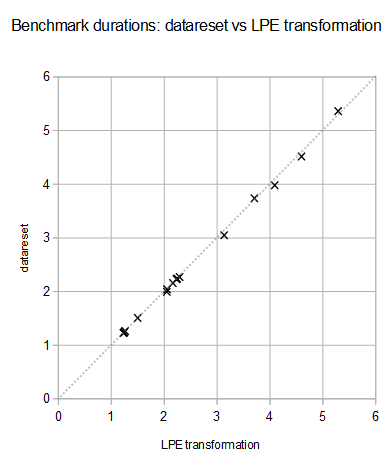
\includegraphics[width=0.7\linewidth]{charts/datareset-vs-lpe-only}
\caption{Benchmark results: datareset vs LPE transformation}
\label{datareset-vs-lpe-only:fig}
\end{center}
\end{figure}


\chapter{parreset}

\section{Introduction}

An LPE may have parameters of which the values are not used anymore after a particular state.
If such parameters can have different values after that state, they continue to add states to the state space for each of those values -- \emph{without} adding any new behavior!

The \texttt{parreset} command tries to determine whether the value of a parameter is used by an LPE after a particular summand.
If this is the case, the parameter is said to be \emph{relevant} for that summand; otherwise, the summand can `reset' the parameter, meaning that it can be assigned a default value.

To determine the relevance of parameters, \texttt{parreset} analyzes the reachability of summands in a generalized, symbolic manner.
\texttt{datareset}, serving a similar purpose, does a control-flow analysis.

\section{Formal background}

\subsection{Possible successors}

Consider all possible pairs of summands of the LPE (including symmetric pairs).
Of a given summand pair $(s, t)$, let $t$ be a \emph{possible successor} of $s$ if the following equation is satisfiable:
\begin{align*}
c_s \land {c_t}[p \rightarrow q(p) \;|\; p \in P][q(p) \rightarrow v_s(p) \;|\; p \in P]
\end{align*}

where

\begin{itemize}
\item $c_s$ and $c_t$ are the guards of summands $s$ and $t$, respectively;
\item $P$ is the set of all LPE parameters;
\item $q(p)$ is a bijective function that relates LPE parameter $p$ to a fresh variable;
\item $v_s(p)$ is the expression that defines the new value of LPE parameter $p$ after the application of summand $s$.
\end{itemize}

The fresh variables of the bijective function $q(p)$ are necessary to distinguish LPE parameters before and after the application of summand $s$ (if $p$ is the LPE parameter before, then $q(p)$ is the LPE parameter after).

\section{Implementation}

The algorithm is a generalization of an existing algorithm \cite{van2009state}.
It consists of two phases.

During the first phase (the preparation phase), we determine all successors of each summand of the LPE using the equation from the previous section.

The second phase (the iteration phase) follows these steps:

\begin{enumerate}

\item For each summand $s$ of the LPE, create a set $R_s$ that contains all parameters of the LPE.
This means that, initially, we assume that all parameters of the LPE are used by one or more of the successors of $s$; that is, \emph{relevant} to $s$.

\item For each summand $s$ of the LPE, set the value of $R_s$ to $\bigcup\limits_{t \in S_s}^{} r(t)$ where $S_s$ is the set of all successors of $s$ (as determined during the preparation phase) and where $r$ is the function
\begin{align*}
r(t) = \left( \text{vars}(c_t) \cup \bigcup\limits_{x \in R_t}^{} \text{vars}(v_t(x)) \right) \setminus C_t
\end{align*}

where

\begin{itemize}
\item $\text{vars}(c_t)$ gives the free variables in $c_t$, the guard of summand $t$;
\item $v_t(p)$ is the expression that defines the value of LPE parameter $p$ after the application of summand $t$;
\item $\text{vars}(v_t)$ gives the free variables in $v_t$;
\item $C_t$ is the set of the communication variables used by summand $t$.
\end{itemize}

\item Repeat the previous step until the fixpoint of $R_s$ is reached for each summand $s$ of the LPE.

\item For each summand $s$ and for all $p \in P \setminus R_s$, change the expression $v_s(p)$ (which defines the value of LPE parameter $p$ after the application of $s$) to $v_I(p)$, the value of $p$ in this initial state of the LPE.

\end{enumerate}

\section{Example TOCHECK}

Consider the following LPE:

\begin{lstlisting}
//Process definition:
PROCDEF example[A :: Int, B](x, y :: Int)
  = A ? i [[x==0]] >-> example[A, B](1, i)
  + A ? i [[x==1 && i==y]] >-> example[A, B](2, y)
  + B [[x==2]] >-> example[A, B](3, y)
  + B [[x==3]] >-> example[A, B](0, y)
  ;

//Initialization:
example[A, B](0, 0);
\end{lstlisting}

Finding the successors of each summand is easy: each summand has exactly one successor, namely the next one, except in case of the fourth summand, where the first summand is the successor.

It is also obvious that $x$ will always be in $R_s$ for each summand $s$, because each summand uses $x$ in its guard.

Process parameter $y$ will always be in $R_{s_1}$, where $s_1$ is the first summand, because $y$ is used in the guard of $s_1$'s successor (the second summand).
After a few iterations, however, $y$ is removed from $R_{s_2}$ to $R_{s_4}$.
This means that $y$ is assigned a default value in the corresponding summands.
Depending on the mood of the SMT solver, this could give

\begin{lstlisting}
//Process definition:
PROCDEF example[A :: Int, B](x, y :: Int)
  = A ? i [[x==0]] >-> example[A, B](1, i)
  + A ? i [[x==1 && i==y]] >-> example[A, B](2, 0)
  + B [[x==2]] >-> example[A, B](3, 0)
  + B [[x==3]] >-> example[A, B](0, 0)
  ;

//Initialization:
example[A, B](0, 0);
\end{lstlisting}





\chapter{confcheck} \label{confcheck}

\section{Introduction}

The \texttt{confcheck} command perform a \emph{confluence analysis} on the LPE in order to determine which \istep{} summands are \emph{confluent}
A confluent \istep{} summand is an \istep{} summand with the property that the possible behavior of a system is the same up to branching bisimulation before and after the application of that summand.

The \texttt{confcheck} command will rename confluent \istep{}s to \cistep{}s.
Afterwards, the \texttt{confelm} command can be used next in order to prioritize \cistep{}s, which may reduce the state space.

\section{Algorithm}

Consider all possible summands pairs, referencing the elements of the summands conform \ref{summandelements}.
Select all pairs $(s_\alpha, s_\beta)$ of which $C_\alpha$ equals \istep{}.

Since it cannot be assumed that
\begin{align*}
\{ x_1(1), \cdots{} x_1(m_1) \} \cap \{ x_2(1), \cdots{} x_2(m_2) \} = \emptyset{}
\end{align*}

a substitution $X$ is introduced such that
\begin{align*}
X = [ x_2(j) \rightarrow q(x_2(j)) \;|\; 1 \leq j \leq m_2 ]
\end{align*}

where $q(x)$ is a surjective function that yields fresh variables.

We also define
\begin{align*}
V_{1} &= [p_j \rightarrow v_1(p_j) \;|\; 1 \leq j \leq k] \\
V_{2} &= [p_j \rightarrow v_2(p_j)[X] \;|\; 1 \leq j \leq k]
\end{align*}

Using the definitions above, a particular \istep{} summand $s_1$ is confluent if the following expression is a tautology for all pairs $(s_1, s_2)$ such that $s_2 \neq s_1$:
\begin{align*}
g_1 \land g_2[X] \rightarrow g_1[V_2] \land g_2[X][V_1] \land \bigwedge\limits_{j=1}^{k} p_j[V_2][V_1] = p_j[V_1][V_2]
\end{align*}

Note that this approach does \emph{not} yield all confluent \istep{} summands (it is an under-approximation).

\section{Example}

Consider the following example:

\begin{lstlisting}
//Process definition:
PROCDEF example[A :: Int](x, y :: Int)
  = A ? i [[x<=9 /\ x==i]] >-> example[A](x+1, y)
  + ISTEP [[y<=9]] >-> example[A](x, y+1)
  ;

//Initialization:
example[A](0, 0);
\end{lstlisting}

Let $s_1$ be the first and $s_2$ the second summand.
Is $s_2$ confluent?

First, since $\{ x_1(1), \cdots{} x_1(m_1) \} \cap \{ x_2(1), \cdots{} x_2(m_2) \} = \emptyset{}$, $X$ can be ignored.

Second, if
\begin{align*}
g_1 \land g_2 \Leftrightarrow (x \leq 9 \land x=i) \land (y \leq 9)
\end{align*}

holds, then
\begin{align*}
g_1[V_2] \land g_2[V_1] &\Leftrightarrow (x \leq 9 \land x=i)[ y \rightarrow y+1 ] \land (y \leq 9)[ x \rightarrow y+1 ] \\
&\Leftrightarrow (x \leq 9 \land x=i) \land (y \leq 9)
\end{align*}

holds as well.

Third, it is the case that
\begin{align*}
x[V_1][V_2] = x+1 = x[V_2][V_1] \\
y[V_1][V_2] = y+1 = y[V_2][V_1]
\end{align*}

Therefore the confluence condition holds, which means that $s_2$ is confluent.

To store the new information about the second summand, the channel is renamed to \cistep{}:

\begin{lstlisting}
//Process definition:
PROCDEF example[A :: Int](x, y :: Int)
  = A ? i [[x<=9 /\ x==i]] >-> example[A](x+1, y)
  + CISTEP [[y<=9]] >-> example[A](x, y+1)
  ;

//Initialization:
example[A](0, 0);
\end{lstlisting}


\chapter{confelm}

\section{Introduction}
One way in which information about confluence can be used before state space generation, is by appending confluent ISTEPs to other summands.
This has the effect that other branches that could follow those summands are ignored, reducing the size of the state space while maintaining its equivalence up to branching bisimulation.

\section{Formal background}

\subsection{Definite successors}

Consider a summand pair $(s_\alpha, s_\beta)$, referencing the elements of $s_\alpha$ and $s_\beta$ conform \ref{summandelements}.
Summand $s_\beta$ is said to be a \emph{definite successor} of $s_\alpha$ if the following expression is a tautology:
\begin{align*}
g_\alpha \rightarrow {g_\beta}[v \mapsto q(v) \;|\; v \in \varsof{g_\beta} \setminus P][p \mapsto v_\alpha(p) \;|\; p \in P]
\end{align*}

where $q(v)$ is a bijective function that relates variable $v$ to a fresh variable.

For a summand $s$, let $D(s)$ be the set of all definite successors of $s$.
By design, $D(s)$ is an under-approximation of the actual successors of $s$.

\section{Algorithm}

The algorithm follows these steps:

\begin{enumerate}

\item Determine which \istep{} summands of the LPE are confluent (see \ref{confcheck}).
Rename the \istep{} channels in confluent \istep{} summands to \cistep{}.

\item For each summand $s_\alpha$, determine $D(s_\alpha)$.
Consider all possible pairs of summands $(s_\alpha, s_\beta)$ such that $s_\beta \in D(s_\alpha)$ and $C_\beta = \cistep{}$, and reference the elements of $s_\alpha$ and $s_\beta$ conform \ref{summandelements}.

Let
\begin{align*}
X = [ x_\beta(j) \mapsto q(x_\beta(j)) \;|\; 1 \leq j \leq m_\beta ]
\end{align*}

where $q(x)$ is a surjective function that yields fresh variables, and let
\begin{align*}
V_\alpha &= [p_j \mapsto v_\alpha(p_j) \;|\; 1 \leq j \leq k]
\end{align*}

Replace $s_\alpha$ by ${s_\alpha}'$, which is defined as
\begin{align*}
{s_\alpha}' = C_\alpha \; &\texttt{?} \; x_\alpha(1) \; \cdots{} \; \texttt{?} \; x_\alpha(m_\alpha) \\
&\texttt{?} \; x_\beta(1)[X] \; \cdots{} \; \texttt{?} \; x_\beta(m_\beta)[X] \\
&[[g_\alpha]] \; \texttt{>->} \; P(v_\beta(p_1)[X][V_1], \cdots{}, v_2(p_k)[X][V_\alpha])
\end{align*}

\item Replace all occurrences of \cistep{} channels with \istep{} channels.
\end{enumerate}

\section{Example}

Consider the following example:

\begin{lstlisting}
//Process definition:
PROCDEF example[A :: Int](x, y :: Int)
  = A >-> example[A]((x+1) mod 3, y)
  + CISTEP >-> example[A](x, (y+1) mod 4)
  ;

//Initialization:
example[A](0, 0);
\end{lstlisting}

The second summand is a \cistep{} summand.
It is also a definite successor of the first summand.
This means that the second summand will be appended to the first summand.

The second summand is also a definite successor of itself.
This means that the second summand will also be appended to itself.

Therefore, the original process is changed to

\begin{lstlisting}
//Process definition:
PROCDEF example[A :: Int](x, y :: Int)
  = A >-> example[A]((x+1) mod 3, (y+1) mod 4)
  + ISTEP >-> example[A](x, (((y+1) mod 4)+1) mod 4)
  ;

//Initialization:
example[A](0, 0);
\end{lstlisting}

\section{Benchmark results TODO}

TODO

\begin{figure}[!ht]
\begin{center}
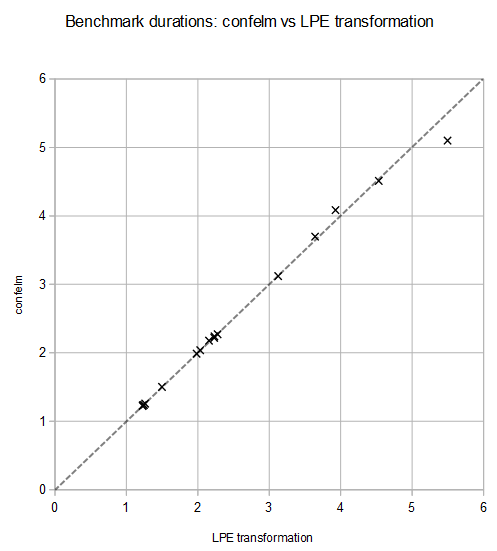
\includegraphics[width=0.7\linewidth]{charts/confelm-vs-lpe-only}
\caption{Benchmark results: confelm vs LPE transformation}
\label{confelm-vs-lpe-only:fig}
\end{center}
\end{figure}




\bibliographystyle{plainnat}
\bibliography{biblio}

\end{document}
